\documentclass[11pt, letterpaper]{memoir}
\usepackage{HomeworkStyle}

\begin{document}
	\begin{center}
		{\large	Quiz 10.2 -- Enthalpies of Phase Change and Heating Curves}
	\end{center}
	{\large Name: \rule[-1mm]{4in}{.1pt} 
		
	\subsection*{Question 1}
	Solid paraffin wax has a specific heat of $2.5\dfrac{J}{g~K}$. If $300.0~J$ of heat are added to $15.25~g$ of paraffin wax, how much will the temperature raise?
	
	\vspace{4.5em}
	\subsection*{Question 2}
	Paraffin wax has a melting point of $37~^\circ C$, and $\Delta H_{fus}=210\dfrac{J}{g}$. How many $J$ of heat are required to melt $5.75~g$ of paraffin wax?
	
	\vspace{4.5em}
	\subsection*{Question 3}
	Sample Exercise 11.3 in Section 11.4 of your textbook gives the necessary values to answer this question
	
	\noindent $38.0~kJ$ of heat are removed from a $10.0~g$ sample of steam (water vapor) at $250.0~^\circ C$. Give the total energy for each of the steps labeled A through E on the cooling curve below, and give the final phase and temperature of the water
	
	
	
	\vspace{12em} 
	\hspace{-3em}\includegraphics[width=0.35\textwidth]{Cooling_Curve}
	
	\newpage
	\pagestyle{empty}
	\addtocounter{page}{-1}
	% \section*{{\fontspec{Microsoft JhengHei}李绅} \emph{(Toiling Farmers)}}
	% \paragraph{By {\fontspec{Microsoft JhengHei}悯农} (Li Shen)}~
	\section*{{\fontspec{AR PL UKai CN}李绅} \emph{(Toiling Farmers)}}
	\paragraph{By {\fontspec{AR PL UKai CN}悯农} (Li Shen)}~
	
	{\fontspec{AR PL UKai CN}
		\begin{verse}
			锄禾日当午,\\
			汗滴禾下土。\\
			谁知盘中餐,\\
			粒粒皆辛苦。
		\end{verse}
	}
	
	\vspace{2em}
	\begin{verse}
		Farmers weeding at noon,\\
		Sweat down the field soon.\\
		Who knows food on a tray\\
		Thanks to their toiling day?
	\end{verse}
\end{document}
